%%%%%%%%%%%%%%%%%%%%%%%%%%%%%%%%%%%%%%%%%%%%%%%%%%%%%%%%%%%%%%%%%%%%%%%%%%%
%% This file is part of the book
%%
%% Algorithmic Graph Theory
%% http://code.google.com/p/graph-theory-algorithms-book/
%%
%% Copyright (C) 2011 David Joyner <wdjoyner@gmail.com>
%% Copyright (C) 2011 Minh Van Nguyen <nguyenminh2@gmail.com>
%%
%% See the file COPYING for copying conditions.
%%%%%%%%%%%%%%%%%%%%%%%%%%%%%%%%%%%%%%%%%%%%%%%%%%%%%%%%%%%%%%%%%%%%%%%%%%%

\documentclass{article}

\usepackage{subfigure}
\usepackage{tikz}
\usepackage{tkz-berge}  %% for drawing combinatorial graphs
\usetikzlibrary{external}
\tikzexternalize{graph-digraph}

\begin{document}

\begin{figure}
%%
%% A graph
\subfigure[]{
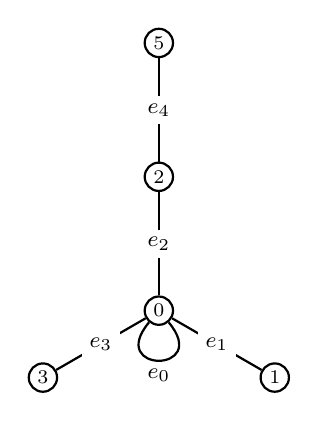
\begin{tikzpicture}
[lineDecorate/.style={-,thick},%
  nodeDecorate/.style={shape=circle,inner sep=1.5pt,draw,thick},%
  scale=1.7]
\scriptsize
%% nodes or vertices
\foreach \nodename/\x/\y in {
  0/0/0, 1/0.8660/-0.5, 2/0/1, 3/-0.8660/-0.5, 5/0/2}
{
  \node (\nodename) at (\x,\y) [nodeDecorate] {$\nodename$};
}
%% edges or lines
\tikzstyle{EdgeStyle}=[-,thick]
\tikzstyle{LabelStyle}=[fill=white]
\foreach \startnode/\endnode/\weight in {0/1/e_1, 0/2/e_2, 0/3/e_3, 2/5/e_4}
{
  \footnotesize
  \Edge[label=$\weight$](\startnode)(\endnode)
}
\path
(0) edge[lineDecorate,loop below,min distance=5mm,out=310,in=230] node {\footnotesize$e_0$} (0);
\end{tikzpicture}
}
\quad
%%
%%
%% A digraph
\subfigure[]{
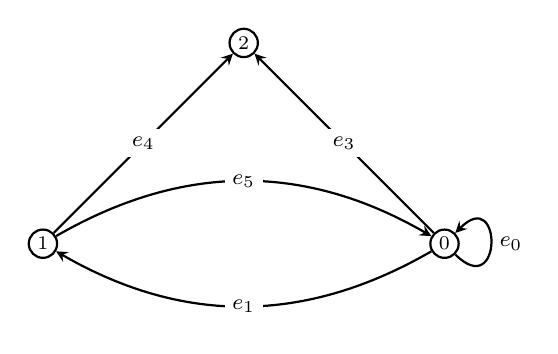
\begin{tikzpicture}
[lineDecorate/.style={-,thick},%
  arrowDecorate/.style={->,>=stealth,thick},%
  nodeDecorate/.style={shape=circle,inner sep=1.5pt,draw,thick},%
  scale=1.7]
\scriptsize
%% nodes or vertices
\foreach \nodename/\x/\y in {0/1.5/0, 1/-1.5/0, 2/0/1.5}
{
  \node (\nodename) at (\x,\y) [nodeDecorate] {$\nodename$};
}
%% edges or lines
\footnotesize
\tikzstyle{EdgeStyle}=[->,>=stealth,thick]
\tikzstyle{LabelStyle}=[fill=white]
\Edge[label=$e_4$](1)(2)
\Edge[label=$e_3$](0)(2)
\Edge[label=$e_1$,style=bend left](0)(1)
\Edge[label=$e_5$,style=bend left](1)(0)
\path
(0) edge[arrowDecorate,loop right,min distance=5mm,out=315,in=45] node {\footnotesize$e_0$} (0);
\end{tikzpicture}
}
\end{figure}

\end{document}
